\chapter{Self-Bounding Algorithms for the Majority Vote}
\label{chap:mv}

\addchapterlof
\addchapterloa
\addchapterloe

\vspace{-1.5cm}
\begin{center}
\textbf{This chapter is based on the following paper}\\[0.1cm]
\end{center}
\printpublication{ViallardGermainHabrardMorvant2021}

\minitoc

\begin{abstract}
As we have seen in \Cref{chap:pac-bayes}, the C-Bound is an insightful upper bound on the risk of a majority vote classifier.
Learning algorithms in the literature minimize the empirical version of the C-Bound, instead of explicit PAC-Bayesian generalization bounds.
In this chapter, we derive self-bounding majority vote learning algorithms to directly optimize PAC-Bayesian guarantees on the C-Bound.
Our algorithms based on gradient descent are scalable and lead to accurate predictors paired with non-vacuous guarantees.
\end{abstract}

\newpage

\section{Introduction}

In this chapter, we introduce new learning algorithms for the majority vote in the context of supervised classification.
The goal of this algorithm is to minimize the true risk of the majority vote.
To do so, one way to minimize such a risk is to minimize the empirical C-Bound~\citep{Breiman2001,LacasseLavioletteMarchandGermainUsunier2006} introduced in \Cref{chap:pac-bayes:sec:surrogate} and estimated on the learning sample $\S$.
This bound has the advantage of involving the performance of the individual voters and the diversity in the voters' set. 
Indeed, these elements are important when one learns a  combination~\citep{Dietterich2000,Kuncheva2014}.
A good majority vote is made up of voters that are ``sufficiently diverse''.\\

Previous algorithms have been developed to minimize the {\it empirical} C-Bound such as \mincq \citep{RoyLavioletteMarchand2011}, \pmincq \citep{BelletHabrardMorvantSebban2014}, \cqboost \citep{RoyMarchandLaviolette2016}, or \cbboost \citep{BauvinCapponiRoyLaviolette2020}.
\citet{RoyLavioletteMarchand2011} first proposed \mincq which consist in minimizing a quadratic problem to learn a majority vote.
\mincq considers a specific voters' set to regularize the minimization process; the algorithm \pmincq generalizes \mincq by allowing prior distributions different from the uniform one.
One  drawback of \mincq and \pmincq is that the optimization problem is not scalable to large datasets.
Lately, \citet{BauvinCapponiRoyLaviolette2020} proposed \cbboost that minimizes in a boosting-based procedure with the advantage to be more scalable while obtaining sparser majority vote.
However, since both \mincq and \cbboost minimize the empirical C-Bound, the PAC-Bayesian generalization bound associated with their learned majority vote predictors can be vacuous.
Note that \cbboost has been proposed to improve another algorithm called  \cqboost~\citep{RoyMarchandLaviolette2016}.
Despite being empirically efficient and justified by theoretical analyses based on the C-Bound, all these methods minimize the empirical C-Bound and not directly a PAC-Bayesian generalization bound on the C-Bound.
This can lead to vacuous generalization bound values and, thus, to poor risk certificates.
When it comes to deriving a learning algorithm that directly minimizes a PAC-Bayesian bound, it is mentioned in the literature that optimizing a PAC-Bayesian bound on the C-bound is not trivial~\citep{MasegosaLorenzenIgelSeldin2020,LorenzenIgelSeldin2019}. 
This underlines the need for other majority vote learning algorithms based on the C-Bound, which motivates our contributions of \Cref{chap:mv:section:contribution}.\\


We cover in this chapter three different PAC-Bayesian viewpoints on generalization bounds for the C-Bound~\citep{McAllester2003,Seeger2002,LacasseLavioletteMarchandGermainUsunier2006}.
We derive three algorithms from these three views to optimize generalization bounds on the C-Bound.
By doing so, we achieve {\it self-bounding algorithms}~\citep{Freund1998}: the predictor returned by the learner comes with a statistically valid risk upper bound. 
Importantly, our algorithms rely on fast gradient descent procedures. 
As far as we know, this is the first work that proposes both efficient algorithms for C-Bound optimization and non-trivial risk-bound values.\\

We provide all the proofs in \Cref{ap:mv} for completeness.

\section{Setting}

We stand in supervised classification by following \Cref{chap:pac-bayes}.
In this context, let $\X \subseteq \Rbb^{\d}$ be a $\d$-dimensional input space, and $\Y$ the label space defined by $\Y=\{-1, +1\}$ (in binary classification) or $\Y=\{1, 2, \dots, \L\}$ (in multi-class classification).
We assume an unknown data distribution $\D$ on $\X{\times}\Y$ and a learning sample  $\S{=}\{(\x_i, \y_i)\}_{i=1}^{\m}$  where each example $(\x_i,\y_i)$ is drawn \iid from $\D$; we denote by $\S\sim\D^\m$ the random draw of such a sample.
Given $\H$ a hypothesis set constituted by voters $\h:\X{\rightarrow}\Y$, and  $\S$, the learner aims to find a weighted combination of the voters from $\H$; a distribution models the weights on $\H$.
To learn such a combination in the PAC-Bayesian framework, we assume a {\it prior} distribution $\P\in\M^{*}(\H)$ on $\H$, and---after the observation of $\S$---we learn a {\it posterior} distribution $\Q\in\M(\H)$ on $\H$.
More precisely, we aim to learn a well-performing classifier that is expressed as a $\Q$-\textit{weighted majority vote} $\MVQ$ defined as 
\begin{align*}
\forall \x\in\X,\quad  \MVQ(\x) \defeq \argmax_{\y'\in\Y} \PP_{\h\sim\Q}\LB \h(\x) = \y'\RB = \argmax_{\y'\in\Y}\EE_{\h\sim\Q}\indic\LB \h(\x) = \y'\RB.
\end{align*}
We thus want to learn $\MVQ$ that  commits as few errors as possible on unseen data from $\D$,
{\it i.e.}, that leads to a low true risk $\Risk_{\D}(\MVQ)$ under the 01-loss defined as
\begin{align*}
\Risk_{\D}(\MVQ) \triangleq \EE_{(\x, \y)\sim\D} \indic\LB \MVQ(\x) \ne \y\RB = \PP_{(\x, \y)\sim\D}\LB \MVQ(\x) \ne \y\RB.
\end{align*}

Since the majority vote's risk is not appealing for optimization (because its gradient is zero everywhere), some surrogates have been introduced (see \Cref{chap:pac-bayes:sec:surrogate}).
For instance, the Gibbs risk (\Cref{chap:pac-bayes:def:gibbs}) is the average risk of the voters and is  defined by
\begin{align*}
r_{\D}(\Q) \defeq \EE_{(\x,\y)\sim\D}   \EE_{\h\sim \Q} \indic\LB\h(\x) \ne \y\RB = \PP_{(\x,\y)\sim\D, \h\sim\Q}\LB \h(\x) \ne \y \RB.
\end{align*}
Unlike the Gibbs risk, the disagreement (\Cref{chap:pac-bayes:def:disagreement}) defined as
\begin{align*}
    d_{\D}(\Q) &\defeq 2\cdot\!  \EE_{(\x,\y)\sim\D}\EE_{\h\sim\Q}\EE_{\h'\sim\Q}\indic\LB \h(\x)\ne \y\RB\indic\LB \h'(\x)=\y\RB,
\end{align*}
\looseness=-1
takes the diversity of the voters into account.
Moreover, the joint error (\Cref{chap:pac-bayes:def:joint}) can be seen as a trade-off between these two quantities.
It is defined as
\begin{align*}
e_{\D}(\Q) &\defeq \EE_{(\x,\y)\sim\D} \EE_{\h\sim\Q}\EE_{\h'\sim\Q}
     \indic\LB\h(\x) \ne \y\big]\indic\big[\h'(\x) \ne \y\RB\\
     &= r_{\D}(\Q)-\frac{1}{2}d_{\D}(\Q).
\end{align*}

By combining these surrogates, one can prove an upper-bound on the majority vote true risk called the C-Bound (\Cref{chap:pac-bayes:theorem:cbound}) and defined as
\begin{align*}
\Risk_{\D}(\MVQ) &\le 1-\frac{\LP1-2r_{\D}(\Q)\RP^2}{1-2d_{\D}(\Q)}\\
&= 1-\frac{\big(1-\LB2e_{\D}(\Q)+d_{\D}(\Q)\RB\big)^2}{1-2d_{\D}(\Q)}.
\end{align*}
However, these surrogates and the C-Bound are not computable because the distribution $\D$ is considered {\it unknown}.
Hence, we need to use PAC-Bayesian generalization bounds in order to upper-bound the majority vote's true risk with a C-Bound based on the empirical counterparts of these surrogates.
Combined with the C-Bound, the PAC-Bayesian theory offers a natural way to analyze the risk of the majority vote.
The principal PAC-Bayesian bounds for the majority vote are recalled in the next section.

\section{State of the Art: PAC-Bayesian Bounds for the Majority Vote}
\label{chap:mv:sec:pb}

This section recalls different PAC-Bayesian bounds upper-bounding the majority vote's true risk.
In particular, we remind two PAC-Bayesian bounds used based on two surrogates from \Cref{chap:pac-bayes:sec:surrogate}: Gibbs risk $r_{\D}(\Q)$ and the joint error $e_{\D}(\Q)$.
Additionally, we recall three PAC-Bayesian bound on the C-Bound, that we call {\it PAC-Bayesian C-Bound}, which is key in our contribution of this chapter. 
Note that the PAC-Bayesian C-Bounds were initially developed for the binary setting but the extension for the multi-class is direct with the $\frac{1}{2}$-margin of \citet{LavioletteMorvantRalaivolaRoy2017}.

\subsection{PAC-Bayesian Bound on the Gibbs Risk}
\label{chap:mv:sec:gibbs}

One PAC-Bayesian bound, originally derived by \citet{GermainLacasseLavioletteMarchandRoy2015}, is based on the Gibbs risk $r_{\D}(\Q)$.
It is recalled in the following theorem.

\begin{restatable}[PAC-Bayesian Bound Based on the Gibbs Risk]{theorem}{theorempbtwogibbs}\label{chap:mv:theorem:pb-2gibbs}
\looseness=-1 For any distribution $\D$ on $\X\times\Y$, for any hypothesis set $\H$, for any distribution $\P\in\M^{*}(\H)$, for any $\delta\in(0,1]$, with probability at least $1-\delta$ over the random choice of $\S\sim\D^\m$ we have
\begin{align}
&\forall\Q\in\M(\H),\quad r_{\D}(\Q) \le \klmax\!\LP r_{\dS}(\Q) \;\middle|\; \frac{1}{\m}\!\LB\KL(\Q\|\P)+\ln\frac{2\sqrt{\m}}{\delta}\RB\RP,\nonumber\\
\text{and}\ &\forall\Q\in\M(\H),\quad \Risk_{\D}(\MVQ) \le 2\LB \klmax\!\LP r_{\dS}(\Q) \;\middle|\; \frac{1}{\m}\!\LB\KL(\Q\|\P)+\ln\frac{2\sqrt{\m}}{\delta}\RB\RP \RB,\label{chap:mv:eq:pb-2gibbs}
\end{align}
where $\klmax(q | \threshold)\defeq\max\Big\{ p \in (0,1) \;\Big|\; \kl(q\|p) \le \threshold\Big\}$ (see \Cref{chap:pac-bayes:subsubsection:seeger-germain}).
\end{restatable}
\begin{noaddcontents}\begin{proof}
Deferred to~\Cref{ap:mv:proof-pb-2gibbs}.
\end{proof}\end{noaddcontents}

However, since the Gibbs risk does not consider the voters' correlation, the majority votes obtained by minimizing this bound do not perform well in practice.
Hence, other PAC-Bayesian bounds have therefore been derived to address this issue.

\subsection{PAC-Bayesian Bound on the Joint Error}

Another PAC-Bayesian bound based on the joint error $e_{\D}(\Q)$ can be derived \citep[Theorem~25]{GermainLacasseLavioletteMarchandRoy2015}.
Compared to \Cref{chap:mv:theorem:pb-2gibbs}, the bound of \Cref{chap:mv:theorem:pb-joint-error} takes better into account the voters' diversity (see \Cref{chap:pac-bayes:sec:surrogate}).

\begin{restatable}[PAC-Bayesian Bound Based on the Joint Error]{theorem}{theorempbjoint}\label{chap:mv:theorem:pb-joint-error}
\looseness=-1
For any distribution $\D$ on $\X\times\Y$, for any hypothesis set $\H$, for any distribution $\P\in\M^{*}(\H)$, for any $\delta\in(0,1]$, with probability at least $1-\delta$ over the random choice of $\S\sim\D^\m$ we have
\begin{align*}
&\forall\Q\in\M(\H),\quad e_{\D}(\Q) \le \klmax\!\LP e_{\dS}(\Q) \;\middle|\; \frac{1}{\m}\!\LB 2\KL(\Q\|\P)+\ln\frac{2\sqrt{\m}}{\delta}\RB\RP,\\
\text{and}\quad &\forall\Q\in\M(\H),\quad \Risk_{\D}(\MVQ) \le 4\LB \klmax\!\LP e_{\dS}(\Q) \;\middle|\; \frac{1}{\m}\!\LB 2\KL(\Q\|\P)+\ln\frac{2\sqrt{\m}}{\delta}\RB\RP \RB.
\end{align*}
\end{restatable}
\begin{noaddcontents}\begin{proof}
Deferred to~\Cref{ap:mv:proof-pb-joint-error}.
\end{proof}\end{noaddcontents}

Note that a looser bound based on the $\kl()$ relaxation of \citet{ThiemannIgelWintenbergerSeldin2017} is presented by \citet{MasegosaLorenzenIgelSeldin2020}.
However, from \Cref{chap:pac-bayes:theorem:relationship}, we know that there is a tighter bound on the majority vote's risk: the C-Bound \citep{Breiman2001,LacasseLavioletteMarchandGermainUsunier2006}.

\subsection{PAC-Bayesian C-Bound of \protect\citeauthor{RoyMarchandLaviolette2016}}

PAC-Bayesian bounds can be used jointly with the C-Bound to obtain a computable bound on the majority vote's true risk; we call such a bound a {\it PAC-Bayesian C-Bound}.
The most intuitive and interpretable PAC-Bayesian C-Bound has been derived by \citet{RoyMarchandLaviolette2016,LavioletteMorvantRalaivolaRoy2017}.
The first proof of this PAC-Bayesian bound has been developed by \citep{RoyMarchandLaviolette2016} in the binary setting; it has been extended to the multi-class setting by \citet[Theorem~3]{LavioletteMorvantRalaivolaRoy2017}.
It consists in upper-bounding separately the Gibbs risk $r_{\D}(\Q)$ and the disagreement $d_{\D}(\Q)$ with the \citeauthor{McAllester2003}'s PAC-Bayesian bound (\Cref{chap:pac-bayes:theorem:mcallester}).
This intuitive PAC-Bayesian bound is recalled in the following theorem.

\begin{restatable}[PAC-Bayesian C-Bound of \citet{RoyMarchandLaviolette2016}]{theorem}{theoremcboundmcallester}\label{chap:mv:theorem:cbound-mcallester}
For any distribution $\D$ on $\X\times\Y$, for any hypothesis set $\H$, for any distribution $\P\in\M^{*}(\H)$, for any $\delta\in(0,1]$, with probability at least $1-\delta$ over the random choice of $\S\sim\D^\m$ we have for all $\Q\in\M(\H)$
\begin{align}
 &\Risk_{\D}(\MVQ) \le \underbrace{1{-}\frac{\LP 1-2\min\LB\frac{1}{2},r_{\dS}(\Q){+}\sqrt{\frac{1}{2\m}\LB \KL(\Q\|\P){+}\ln\tfrac{4\sqrt{\m}}{\delta}\RB}\RB\RP^2}{1-2\max\LB 0, d_{\dS}(\Q){-}\sqrt{\frac{1}{2\m}\LB 2\KL(\Q\|\P){+}\ln\tfrac{4\sqrt{\m}}{\delta}\RB}\RB}}_{{\displaystyle\defeq\ \MCBound}}.\label{chap:mv:eq:cbound-mcallester}
\end{align}
\end{restatable}
\begin{noaddcontents}\begin{proof}
Deferred to~\Cref{ap:mv:sec:proof-cbound-mcallester}.
\end{proof}\end{noaddcontents}

While there is no algorithm that directly minimizes \Cref{chap:mv:theorem:cbound-mcallester}, this kind of interpretable bound can be seen as a justification of the optimization of $r_{\dS}(\Q)$ and $d_{\dS}(\Q)$ in the empirical C-Bound such as for \mincq~\citep{RoyLavioletteMarchand2011} or \cbboost~\citep{BauvinCapponiRoyLaviolette2020}.
In \Cref{chap:mv:section:contribution-mcallester}, we derive the first algorithm to directly minimize it.

However, this PAC-Bayesian C-Bound can have a severe disadvantage with a small $\m$ and a Gibbs risk close to $\tfrac{1}{2}$: even for a $\KL(\Q\|\P)$ close to $0$, the value of the PAC-Bayesian C-Bound will be close to $1$.
To overcome this drawback, one solution is to follow another tighter PAC-Bayesian bound, the one proposed by \citet{Seeger2002} (\Cref{chap:pac-bayes:theorem:seeger}).
%
Actually, we further recall two bounds based on this approach: the first one in \Cref{chap:mv:theorem:cbound-seeger} involves the Gibbs risk $r_{\dS}(\Q)$ and the disagreement $d_{\dS}(\Q)$ (as \Cref{chap:mv:theorem:cbound-mcallester}) and the second one in \Cref{chap:mv:theorem:cbound-lacasse} involves the joint error $e_{\dS}(\Q)$ and the disagreement $d_{\dS}(\Q)$.  

\subsection{PAC-Bayesian C-Bound of \protect\citeauthor{GermainLacasseLavioletteMarchandRoy2015}}

The PAC-Bayesian generalization bounds based on the \citeauthor{Seeger2002}'s approach are known to produce tighter bounds.
As for \Cref{chap:mv:theorem:cbound-mcallester}, the result below bounds independently the Gibbs risk $r_{\D}(\Q)$ and the disagreement $d_{\D}(\Q)$; see the PAC-Bound 1 of \citet{GermainLacasseLavioletteMarchandRoy2015}.
Note that \citet{GermainLacasseLavioletteMarchandRoy2015} proved the bound for the binary setting but the multi-class setting is also handled.
It is recalled in the following theorem.

\begin{restatable}[PAC-Bayesian C-Bound of~\citet{GermainLacasseLavioletteMarchandRoy2015}]{theorem}{theoremcboundseeger}\label{chap:mv:theorem:cbound-seeger}
For any distribution $\D$ on $\X\times\Y$, for any hypothesis set $\H$, for any distribution $\P\in\M^{*}(\H)$, for any $\delta\in(0,1]$, with probability at least $1-\delta$ over the random choice of $\S\sim\D^\m$ we have for all $\Q\in\M(\H)$
\begin{align}
\Risk_{\D}(\MVQ) \le \underbrace{1{-}\frac{\Bigg(1{-}2\min\Big[\frac{1}{2},  \klmax \LP r_{\dS}(\Q) \;\middle|\; \frac{1}{\m}\LB \KL(\Q\|\P){+}\ln\tfrac{4\sqrt{\m}}{\delta}\RB\RP\Big]\Bigg)^2}{1{-}2\max\Bigg[ 0,
\klmin\LP d_{\dS}(\Q) \;\middle|\; \frac{1}{\m}\LB 2\KL(\Q\|\P){+}\ln\tfrac{4\sqrt{\m}}{\delta}\RB\RP\Bigg]}}_{\displaystyle\defeq\ \SCBound}.\label{chap:mv:eq:cbound-seeger}
\end{align}
\end{restatable}
\begin{noaddcontents}\begin{proof}
Deferred to~\Cref{ap:mv:sec:proof-cbound-seeger}.
\end{proof}\end{noaddcontents}

\looseness=-1
Note that this PAC-Bayesian C-Bound is tighter than \Cref{chap:mv:eq:cbound-mcallester} because the \citeauthor{Seeger2002}'s PAC-Bayesian bound is tighter than the one of \citeauthor{McAllester2003}'s one (see \Cref{chap:pac-bayes:sec:pac-bayes}).
However, one drawback of this PAC-Bayesian C-Bound is that the Gibbs risk 
$r_{\D}(\Q)$ and the disagreement $d_{\D}(\Q)$ are upper-bounded independently.

\subsection{PAC-Bayesian C-Bound of \protect\citeauthor{LacasseLavioletteMarchandGermainUsunier2006}}
\label{chap:mv:section:pac-bayesian-e-d}

\citet{LacasseLavioletteMarchandGermainUsunier2006} proposed to bound simultaneously the joint error $e_{\D}(\Q)$ and the disagreement $d_{\D}(\Q)$.
Here, to compute the bound, we need to find the worst C-Bound value that can be obtained with a couple of joint error and disagreement denoted by $(e,d)$ belonging to the set $\Abb_{\dS}(\Q)$ that is defined by
\begin{align*}
\Abb_{\dS}(\Q) = \Bigg\{ (e, d) \;\Big|\; &\kl\LP e_{\dS}(\Q),  d_{\dS}(\Q)\|e, d\RP \le \frac{1}{\m}\LB 2\KL(\Q\|\P) + \ln\tfrac{2\sqrt{\m}+\m}{\delta}\RB,\\
&\hspace{0.1cm}d\le 2 \sqrt{e}{-}2e\,,\ 2e{+}d<1\Bigg\},\\
&\hspace{-2.1cm}\text{where}\quad \kl(q_1{,} q_2\| p_1{,} p_2) = q_1\ln\!\frac{q_1}{p_1} + q_2 \ln\!\frac{q_2}{p_2} + (1{-}q_1{-}q_2)\ln\!\frac{1{-}q_1{-}q_2}{1{-}p_1{-}p_2}.
\end{align*}
Based on $\Abb_{\dS}(\Q)$, \citet{LacasseLavioletteMarchandGermainUsunier2006} derive the following PAC-Bayesian C-Bound. 

\begin{restatable}[PAC-Bayesian C-Bound of \citet{LacasseLavioletteMarchandGermainUsunier2006}]{theorem}{theoremcboundlacasse}\label{chap:mv:theorem:cbound-lacasse}
For any distribution $\D$ on $\X\times\Y$, for any hypothesis set $\H$, for any distribution $\P\in\M^{*}(\H)$, for any $\delta\in(0,1]$, with probability at least $1-\delta$ over the random choice of $\S\sim\D^\m$ we have for all $\Q\in\M(\H)$
\begin{align*}
&\hspace{-1cm}\Risk_{\D}(\MVQ) \le \sup_{(e, d)\in \Abb_{\dS}(\Q)} \LB 1- \frac{\LP 1-(2e+d)\RP^2}{1-2d} \RB,\\
\text{where}\quad \Abb_{\dS}(\Q) = \Bigg\{ (e, d) \;\Big|\; &\kl\LP e_{\dS}(\Q),  d_{\dS}(\Q)\|e, d\RP \le \frac{1}{\m}\LB 2\KL(\Q\|\P) + \ln\tfrac{2\sqrt{\m}+\m}{\delta}\RB,\\
&d\le 2 \sqrt{e}{-}2e\,,\ 2e{+}d<1\Bigg\}.
\end{align*}
\end{restatable}
\begin{noaddcontents}\begin{proof}
Deferred to~\Cref{ap:mv:sec:proof-cbound-lacasse}.
\end{proof}\end{noaddcontents}

This PAC-Bayesian C-Bound can be more challenging to compute: it requires to solve a (convex) optimization problem to obtain a bound value.

\section{Contribution: Algorithms based on the PAC-Bayesian C-Bounds}
\label{chap:mv:section:contribution}

In this section, we present three self-bounding algorithms minimizing directly the PAC-Bayesian C-Bounds introduced previously.

\subsection{Algorithm based on \Cref{chap:mv:eq:cbound-mcallester}}

\label{chap:mv:section:contribution-mcallester}
\begin{algorithm}[H]
  \caption{Minimization of \Cref{chap:mv:eq:cbound-mcallester} by Stochastic Gradient Descent}
  \begin{algorithmic}
    \State{{\bf Given: } learning sample $\S$, prior distribution $\P\in\M^{*}(\H)$, the objective function $\MObj$}
    \State{{\bf Hyperparameters: } number of iterations $\iter$}
    \State{$\Q \leftarrow \P$}
    \For{$\t\leftarrow 1$ to $\iter$}
    \For{{\bf all} mini-batches $\batch\subseteq\S$}
    \State{$\Q\leftarrow$ Update $\Q$ with $\MObjbatch$ by gradient descent\footnotemark}
    \EndFor
    \EndFor    
    \State{\Return{$\Q$}}
  \end{algorithmic}
  \label{chap:mv:algo:mcallester}
\end{algorithm}
\footnotetext{The update of $\Q$ can be done with a vanilla gradient descent or with the update of another algorithm like Adam~\citep{KingmaBa2015} or COCOB~\citep{OrabonaTommasi2017}.} 

We derive in \Cref{chap:mv:algo:mcallester} a method to directly minimize the  PAC-Bayesian C-Bound of \Cref{chap:mv:theorem:cbound-mcallester} by stochastic gradient descent.
An important aspect of the optimization is that if $r_{\dS}(\Q){+}{\scriptstyle\sqrt{\frac{1}{2\m}[ \KL(\Q\|\P){+}\ln{\scriptscriptstyle\frac{4\sqrt{\m}}{\delta}}]}}\ge \frac{1}{2}$, the gradient of the numerator in $\MCBound$ with respect to $\Q$ is 0 which makes the optimization impossible.
Hence, we aim to minimize the following constraint optimization problem:
\begin{align*}
    \min_{\Q\in\M(\H)}&\underbrace{\LC 1{-}\frac{\LP 1-2\min\LB\frac{1}{2},r_{\dS}(\Q){+}\sqrt{\frac{1}{2\m}\LB \KL(\Q\|\P){+}\ln\tfrac{4\sqrt{\m}}{\delta}\RB}\RB\RP^2}{1-2\max\LB 0, d_{\dS}(\Q){-}\sqrt{\frac{1}{2\m}\LB 2\KL(\Q\|\P){+}\ln\frac{4\sqrt{\m}}{\delta}\RB}\RB}\RC}_{\displaystyle\defeq\ \MCBound}\\
    \quad&\text{s.t }\quad r_{\dS}(\Q){+}\sqrt{\frac{1}{2\m}\LB \KL(\Q\|\P){+}\ln\tfrac{4\sqrt{\m}}{\delta}\RB}\le\frac{1}{2}.
\end{align*}
From this formulation, we deduce a non-constrained optimization problem:
\begin{align*}
\min_{\Q\in\M(\H)}\LC \MCBound + \logbar\!\LB r_{\dS}(\Q){+}\sqrt{\frac{1}{2\m}\LB \KL(\Q\|\P){+}\ln\frac{4\sqrt{\m}}{\delta}\RB}{-}\frac{1}{2}\RB\RC,
\end{align*}
where $\logbar()$ is the barrier function defined as $\logbar(a)\!=\!0$ if $a\!\le\! 0$ and $\logbar(a)\!=\!+\infty$ otherwise.
Due to the nature of $\logbar()$, this problem is not suitable for optimization: the objective function will be infinite when $a\!>\!0$.
To tackle this drawback, we replace $\logbar()$ by the approximation introduced by~\citet{KervadecDolzYuanDesrosiersGrangerAyed2019} called the log-barrier extension and defined as 
\begin{align*}
    \logbar_{\lambda}(a) = \left\{\begin{array}{cc}
        -\tfrac{1}{\lambda}\ln(-a), & \text{if } a \le -\tfrac{1}{\lambda^2}, \\[1mm]
        \lambda a{-}\tfrac{1}{\lambda}\ln(\tfrac{1}{\lambda^2}){+}\tfrac{1}{\lambda}, & \text{otherwise.}
    \end{array}\right.
\end{align*}

\begin{figure}
    \centering
    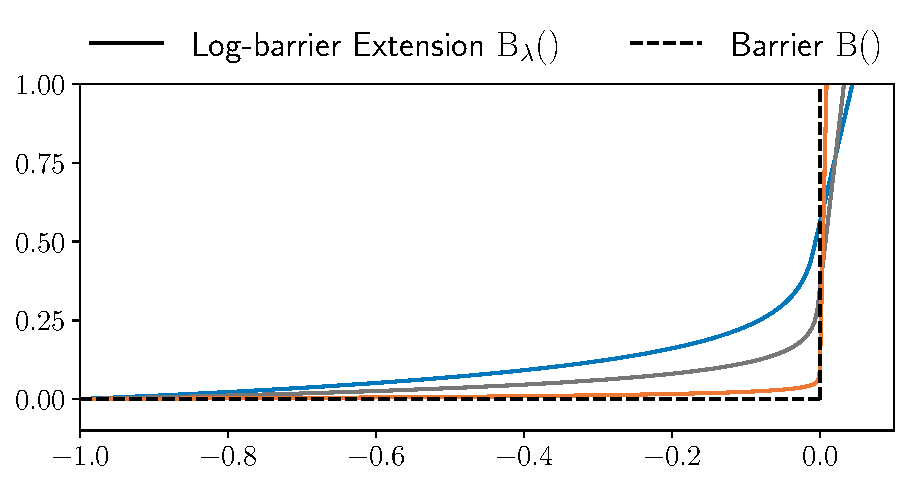
\includegraphics[width=0.8\linewidth]{chapter_4/figures/log_barrier.pdf}
    \caption[]{
    Plot of the barrier function $\logbar()$ (with the dotted line) and the log-barrier extension $\logbar_{\lambda}()$ (plain lines).
    We plot the function with three parameters: $\lambda \in \{10, 20, 100\}$.
    The higher the parameter $\lambda$, the closer the function $\logbar_{\lambda}()$ to the barrier function $\logbar()$. 
    Thus, the blue, gray and orange curves are respectively with the parameter $\lambda=10$, $\lambda=20$ and $\lambda=100$.
    }
    \label{chap:mv:fig:log_barrier}
\end{figure}

\looseness=-1
The parameter $\lambda\in\R_{*}^{+}$ parameterized the log-barrier extension $\logbar_{\lambda}()$.
The function $\logbar_{\lambda}()$ tends to $\logbar()$ when $\lambda$ tends to $+\infty$; we plot in \Cref{chap:mv:fig:log_barrier} these two functions.
Compared to the standard log-barrier\footnote{The reader can refer to \citet{BoydVandenberghe2014} for an introduction of standard log-barrier and interior-point methods.}, the function $\logbar_{\lambda}()$ is differentiable even when the constraint is not satisfied, \ie, when $a > 0$.
Thanks to $\logbar_{\lambda}()$, we can take the constraint $r_{\dS}(\Q){+}{\scriptstyle\sqrt{\frac{1}{2\m}[ \KL(\Q\|\P){+}\ln{\scriptscriptstyle\frac{4\sqrt{\m}}{\delta}}]}}\le\!\tfrac{1}{2}$ into account.
Moreover, when the number of examples $\m$ is large, we estimate the PAC-Bayesian C-Bound $\MCBound$ and the Gibbs risk $r_{\dS}(\Q)$ with a mini-batch $\batch\subseteq\S$.
Concretely, our objective function that is minimized by stochastic gradient descent with \Cref{chap:mv:algo:mcallester} is the following:
\begin{align*}
   \MObjbatch \ =\ \MCBoundbatch + \logbar_{\lambda}\LB r_{\dbatch}(\Q){+}\sqrt{\frac{1}{2\m}\LB \KL(\Q\|\P){+}\ln\frac{4\sqrt{\m}}{\delta}\RB}{-}\frac{1}{2}\RB.
\end{align*}
For a given $\lambda$, the optimizer will find a solution with a good trade-off between minimizing $\MCBoundbatch$ and the log-barrier extension function $\logbar_{\lambda}()$.
As shown in the experiments, minimizing the \citeauthor{McAllester2003}-based bound does not lead to the tightest bound.
Indeed, such a bound is looser than \citeauthor{Seeger2002}-based bounds and leads to a looser PAC-Bayesian C-Bound. 
\subsection{Algorithm based on \Cref{chap:mv:eq:cbound-seeger}}

In order to obtain better generalization guarantees, we should optimize the \citeauthor{Seeger2002}-based C-bound of \Cref{chap:mv:theorem:cbound-seeger}. 
Hence to minimize such a PAC-Bayesian C-Bound, we seek to minimize the following optimization problem:
\begin{align*}
    \min_{\Q\in\M(\H)}& \underbrace{\LC 1{-}\frac{\LP1{-}2\min\LB\frac{1}{2},  \klmax \LP r_{\dS}(\Q) \;\middle|\; \frac{1}{\m}\LB \KL(\Q\|\P){+}\ln\tfrac{4\sqrt{\m}}{\delta}\RB\RP\RB\RP^2}{1{-}2\max\LB 0,
\klmin\LP d_{\dS}(\Q) \;\middle|\; \frac{1}{\m}\LB 2\KL(\Q\|\P){+}\ln\tfrac{4\sqrt{\m}}{\delta}\RB\RP\RB}\RC}_{\displaystyle \defeq\ \SCBound}\\
&\text{s.t }\quad \klmax \LP r_{\dS}(\Q) \;\middle|\; \tfrac{1}{\m}\!\LB \KL(\Q\|\P){+}\ln\tfrac{4\sqrt{\m}}{\delta}\RB\RP\le\frac{1}{2}.
\end{align*}
For the same reasons as for deriving \Cref{chap:mv:algo:mcallester}, we propose to solve by stochastic gradient descent with a mini-batch $\batch\subseteq\S$:
\begin{align*}
\SObjbatch = \SCBoundbatch + \logbar_{\lambda}\LB\klmax \LP r_{\dbatch}(\Q) \;\middle|\; \tfrac{1}{\m}\!\LB \KL(\Q\|\P){+}\ln\tfrac{4\sqrt{\m}}{\delta}\RB\RP-\frac{1}{2}\RB.
\end{align*}
The main challenge in optimizing it is to evaluate $\klmax$ or $\klmin$ and to compute their derivatives.
The evaluation of $\klmax$ or $\klmin$ is done by \Cref{chap:pac-bayes:algo:kl} proposed by~\citet{ReebDoerrGerwinnRakitsch2018}.
This method consists in refining iteratively an interval $[p_{\text{min}}, p_{\text{max}}]$ with \mbox{$p\in [p_{\text{min}}, p_{\text{max}}]$} such that \mbox{$\kl(q\|p)\!=\!\psi$}.
Moreover, to compute the derivatives with respect to the posterior $\Q$, we use the chain rule for differentiation with a deep learning framework (such as \pytorch~\citep{Paszke2019}) and the derivatives in \Cref{chap:pac-bayes:eq:deriv-kl}. 
The global algorithm is summarized in \Cref{chap:mv:algo:seeger}.

\subsection{Algorithm based on \Cref{chap:mv:theorem:cbound-lacasse}}

\label{section:contribution-e-d}
\Cref{chap:mv:theorem:cbound-lacasse} jointly upper-bounds the joint error $e_{\D}(\Q)$ and the disagreement $d_{\D}(\Q)$; But as pointed out in \Cref{chap:mv:section:pac-bayesian-e-d} its optimization can be hard.
To ease its manipulation, we derive below a C-Bound resulting of a reformulation of the constraints involved in the set $\Abb_{\dS}(\Q)$.

\begin{algorithm}[H]
 \caption{Minimization of \Cref{chap:mv:eq:cbound-seeger} by Stochastic Gradient Descent}
  \begin{algorithmic}
  \State{{\bf Given: } learning sample $\S$,  prior distribution $\P\in\M^{*}(\H)$, the objective function $\SObj$}
    \State{{\bf Hyperparameters: } 
    number of iterations $\iter$}
    \State{$\Q \leftarrow \P$}
    \For{$\t\leftarrow 1$ to $\iter$}
        \For{{\bf all} mini-batches $\batch\subseteq\S$}
            \State{Compute $\SObjbatch$ using \Cref{chap:pac-bayes:algo:kl}}
            \State{$\Q\leftarrow$ Update $\Q$ with $\SObjbatch$ by gradient descent}
        \EndFor
    \EndFor
    \State{\Return{$\Q$}}
  \end{algorithmic}
  \label{chap:mv:algo:seeger}
\end{algorithm}

\begin{restatable}[Reformulation of \citeauthor{LacasseLavioletteMarchandGermainUsunier2006}'s PAC-Bayesian C-Bound]{theorem}{theoremnewcboundlacasse}
For any distribution $\D$ on $\X\times\Y$, for any hypothesis set $\H$, for any distribution $\P\in\M^{*}(\H)$, for any $\delta\in(0,1]$, with probability at least $1-\delta$ over the random choice of $\S\sim\D^\m$ we have for all $\Q\in\M(\H)$
\begin{align}
    &\Risk_{\D}(\MVQ) \le \sup_{(e, d)\in \Abb'_{\dS}(\Q)} \LB 1- \frac{\LP 1-(2e+d)\RP^2}{1-2d} \RB,\label{chap:mv:eq:new-cbound-lacasse}\\ 
    \Abb'_{\dS}(\Q) = \Bigg\{ (e, d) \;\Big|\; &\kl\LP e_{\dS}(\Q),  d_{\dS}(\Q)\|e, d\RP \le \frac{1}{\m}\LB 2\KL(\Q\|\P) + \ln\tfrac{2\sqrt{\m}+\m}{\delta}\RB,\nonumber\\
&d\le 2\sqrt{\min\LP e, \tfrac{1}{4}\RP}{-}2e,\  d<\tfrac{1}{2}\Bigg\}\nonumber.
   \end{align}
\label{chap:mv:theorem:new-cbound-lacasse}
\end{restatable}
\begin{noaddcontents}\begin{proof}
Deferred to~\Cref{ap:mv:sec:proof-new-cbound-lacasse}.
\end{proof}\end{noaddcontents}

\Cref{chap:mv:theorem:new-cbound-lacasse} suggests then the following constrained optimization problem: 
\begin{align*}
    &\min_{\Q\in\M(\H)}\!\left\{\! \sup_{\scalebox{0.8}{$(e{,}d){\in}\!\LB0,\!\tfrac{1}{2}\RB^2$}}\!\!
    \LP 1\!-\! \frac{\big[ 1\!-\!(2e\!+\!d)\big]^2}{1\!-\!2d}\! \RP\,   \text{s.t.}\,  (e, d)\! \in\! \Abb'_{\dS}(\Q) \! \right\} \!\text{ s.t. } 2e_{\dS}(\Q){+}d_{\dS}(\Q)\!\le\! 1,
\end{align*}
Actually, we can rewrite this constrained optimization problem into an unconstrained one using the barrier function. 
We obtain
\begin{align}
    \min_{\Q\in\M(\H)} \Bigg\{&\max_{\scalebox{0.8}{$(e{,}d){\in}\!\LB0,\!\tfrac{1}{2}\RB^2$}}  \Bigg(
     \CBound^{\tt L}(e,d) - \logbar\!\LB d {-} 2\sqrt{\min\LP e, \tfrac{1}{4}\RP}{-}2e\RB -\logbar\!\LB d{-}\tfrac{1}{2}\RB \nonumber\\
     &- \logbar\LB\kl\LP e_{\dS}(\Q),  d_{\dS}(\Q)\|e, d\RP{-}\frac{1}{\m}\LB 2\KL(\Q\|\P) + \ln\tfrac{2\sqrt{\m}+\m}{\delta}\RB\RB
   \Bigg)\nonumber\\
   &+ \logbar\Big[ 2e_{\dS}(\Q){+}d_{\dS}(\Q){-}1\Big]\Bigg\}, \label{eq:k_Q_param_nu}
\end{align}
where $\CBound^{\tt L}(e,d)=1-\tfrac{\LP 1-(2e+d)\RP^2}{1-2d}$ if $d\!<\!\frac12$, and $\CBound^{\tt L}(e,d)\!=\!1$ otherwise.
However, this problem cannot be optimized directly by stochastic gradient descent.
In this case, we have a \mbox{min-max} optimization problem, \ie, for each descent step we need to find the couple $(e, d)$ that maximizes the $\CBound^{\tt L}(e,d)$ given the three constraints that define $\Abb'_{\dS}(\Q)$ before updating the posterior distribution $\Q$.

First, to derive our optimization procedure, we focus on the inner maximization problem when $e_{\dS}(\Q)$ and $d_{\dS}(\Q)$ are fixed in order to find the optimal $(e,d)$.
However, the function $\CBound^{\tt L}(e,d)$ we aim at maximizing is not concave for all $(e,d)\!\in\!\R^2$, implying that the  implementation of its maximization can be hard\footnote{For example, when using \cvxpy~\citep{DiamondBoyd2016}, that uses Disciplined Convex Programming (DCP~\citep{GrantBoydYe2006}), the maximization of a non-concave function is not possible.}. 
Fortunately, $\CBound^{\tt L}(e,d)$ is quasi-concave~\citep{GermainLacasseLavioletteMarchandRoy2015} for $(e, d)\in[0, 1]\times[0, \frac{1}{2}]$.
Then by  definition of quasi-concavity, we have:
\begin{align*}
&\forall \alpha\in [0,1],\quad \left\{ (e, d) \,\middle|\, 1- \frac{\big[ 1-(2e+d)\big]^2}{1-2d} \ge 1-\alpha \right\}\\
\Longleftrightarrow\quad  &\forall \alpha\in [0,1],\quad  \left\{ (e, d) \ \middle|\  
\alpha(1{-}2d)-\Big[1{-}(2e{+}d)\Big]^2 \ge 0\right\}.
\end{align*}

\begin{algorithm}[t]
  \caption{Minimization of \Cref{chap:mv:eq:new-cbound-lacasse} by Stochastic Gradient Descent}
  \begin{algorithmic}
    \State{{\bf Given: } learning sample $\S$, prior $\P\in\M^{*}(\H)$, the objective function $\LObj$}
    \State{{\bf Hyperparameters: }
    number of iterations $\iter$}
    \State{$\Q \leftarrow \P$}
    \For{$\t\leftarrow 1$ to $\iter$}
        \For{{\bf all} mini-batches $\batch\subseteq\S$}
        \State{$(e^*, d^*) \leftarrow $\Call{maximize-$e$-$d$}{$e_{\dbatch}(\Q), d_{\dbatch}(\Q)$}}
        \State{$\Q\leftarrow$ Update $\Q$ with $\LObjbatch$ by gradient descent}
        \EndFor
    \EndFor
    \State{\Return{$\Q$}}\\
    {\centerline{\rule{0.75\linewidth}{0.25pt}}}
      \State{{\bf Given:} learning sample $\S$, joint error $e_{\dS}(\Q)$, disagreement $d_{\dS}(\Q)$}
\State{{\bf Hyperparameters: }tolerance $\epsilon$}
\Function{maximize-$e$-$d$}{$e_{\dS}(\Q), d_{\dS}(\Q)$}
\State{$\alpha_{\text{min}} = 0$ and $\alpha_{\text{max}}=1$}
\While{$\alpha_{\text{max}}-\alpha_{\text{min}}>\epsilon$}
\State{$\alpha=\tfrac{1}{2}(\alpha_{\text{min}}+\alpha_{\text{max}})$}
\State{$(e, d) \leftarrow$ Solve \Cref{chap:mv:eq:min-e-d}}
\State{\textbf{if} $\CBound^{\tt L}(e,d) \ge 1{-}\alpha$ \textbf{then} $\alpha_{\text{max}} \leftarrow \alpha$ \textbf{else} $\alpha_{\text{min}} \leftarrow \alpha$}
\EndWhile
\State{\Return{$(e, d)$}}
\EndFunction
\end{algorithmic}
\label{chap:mv:algo:lacasse}
\end{algorithm}
\noindent Hence, for any fixed $\alpha\!\in\![0, 1]$ we can look for $(e, d)$ that maximizes $\CBound^{\tt L}(e,d)$ and respects the constraints involved in $\Abb'_{\dS}(\Q)$.
This is equivalent to solving the following problem for a given $\alpha\in[0, 1]$:
\begin{align}
    \max_{(e, d)\in[0, \frac{1}{2}]^2}\quad  &\alpha(1{-}2d)-\Big[1{-}(2e{+}d)\Big]^2\label{chap:mv:eq:min-e-d}\\
    \text{ s.t. } d&\le 2\sqrt{\min\LP e, \tfrac{1}{4}\RP}{-}2e\nonumber\\
    \text{ and }\kl\big( e_{\dS}(\Q),  d_{\dS}(\Q)\|e, d&\big)\le \frac{1}{\m}\LB 2\KL(\Q\|\P) + \ln\tfrac{2\sqrt{\m}+\m}{\delta}\RB\nonumber.
\end{align}
In fact, we aim at finding $\alpha\in[0,1]$ such that the maximization of \Cref{chap:mv:eq:min-e-d} leads to $1{-}\alpha$ equals to the largest value of $C^{\tt L}(e, d)$ under the constraints.
To do so, we make use of the ``Bisection method for quasi-convex optimization''~\citep{BoydVandenberghe2014} that is summarized in  \textsc{maximize-$e$-$d$} in \Cref{chap:mv:algo:lacasse}.
We denote by $(e^{*\!}, d^*)$ the solution of \Cref{chap:mv:eq:min-e-d}.
Note that, in practice, the joint error and the disagreement is approximated through the mini-batch $\batch\subseteq\S$.
It remains then to solve the outer minimization problem that becomes:
\begin{align*}
    \min_{\Q\in\M(\H)}\Bigg\{\ &\logbar\LB 2e_{\dS}(\Q){+}d_{\dS}(\Q){-}1\RB\\
    &-\logbar\LB\kl\LP e_{\dS}(\Q),  d_{\dS}(\Q)\|e^{*\!}, d^*\RP{-}\frac{1}{\m}\LB 2\KL(\Q\|\P) + \ln\tfrac{2\sqrt{\m}+\m}{\delta}\RB\RB\ \Bigg\}.
\end{align*}
To obtain a objective function that is suitable for stochastic gradient descent, we bring two modifications to the outer minimization problem: {\it (i)} we replace $\logbar()$ by the log-barrier extension $\logbar_\lambda()$ and {\it (ii)} we approximate the disagreement and the joint error with a mini-batch $\batch\subseteq\S$.
Hence, we obtain the following objective function: 
\begin{align*}
   \LObjbatch = & \logbar_{\lambda}\LB 2e_{\dbatch}(\Q){+}d_{\dbatch}(\Q){-}1\RB
   \\
    &\hspace{-1cm}-\logbar_\lambda \LB\kl\LP e_{\dbatch}(\Q),d_{\dbatch}(\Q)\|e^{*\!},d^*\RP{-}\frac{1}{\m}\LB 2\KL(\Q\|\P) + \ln\tfrac{2\sqrt{\m}+\m}{\delta}\RB\RB.
\end{align*}
The global method is summarized in \Cref{chap:mv:algo:lacasse}.
\noindent As a side note, we  mention that the classic Danskin Theorem~\citep{Danskin1966} used in min-max optimization theory is not applicable in our case since our objective function is not differentiable for all $(e, d)\in[0, \tfrac{1}{2}]^2$. 
We discuss this point in \Cref{ap:mv:sec:danskin}.

\section{Experiments}
\label{chap:mv:sec:expe}

\subsection{Setting}

\begin{figure}
    \centering
    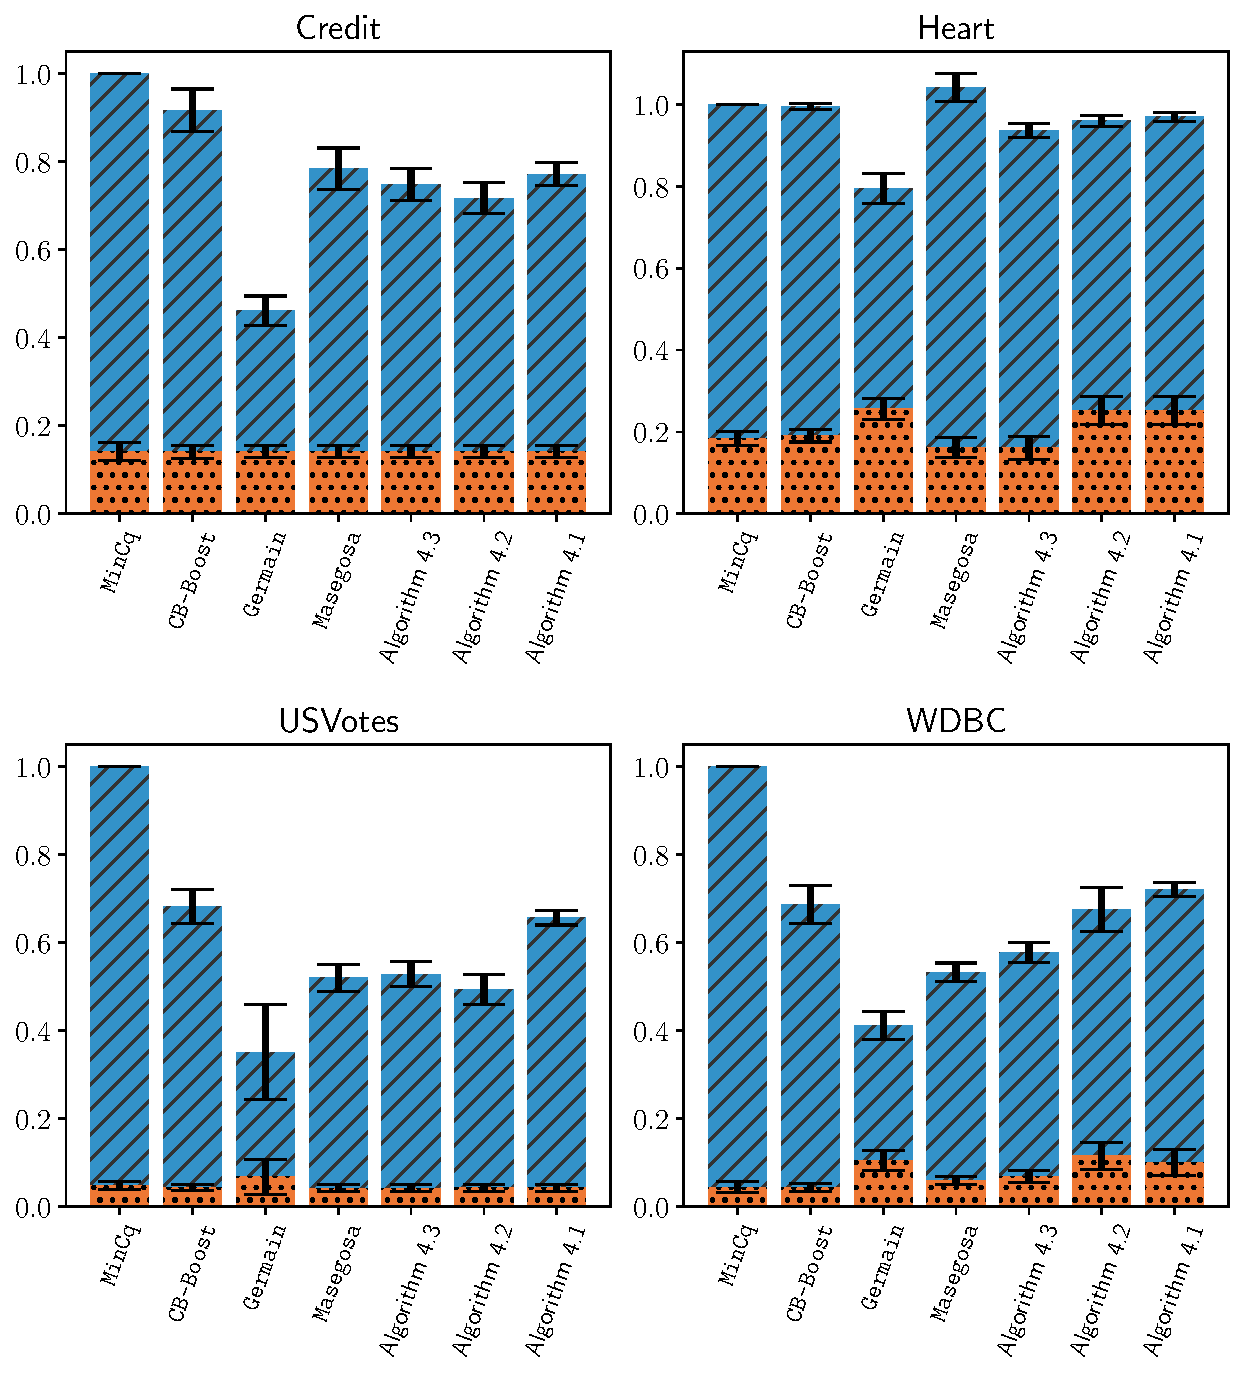
\includegraphics[width=1.0\linewidth]{chapter_4/figures/stump_binary_1.pdf}
    \caption[Comparison Between the Test Risks and the Bounds (1/6)]{
    Plot of a comparison between the test risks $\Risk_{\dT}(\MVQ)$ and the generalization bounds in the binary setting when the voters are decision stumps.
    For each algorithm, we represent the mean of the test risks in the orange bars and the bounds' mean in the blue bars.
    Additionally, the black lines are the standard deviations. 
    }
    \label{chap:mv:fig:stump-binary-1}
\end{figure}

\begin{figure}
    \centering
    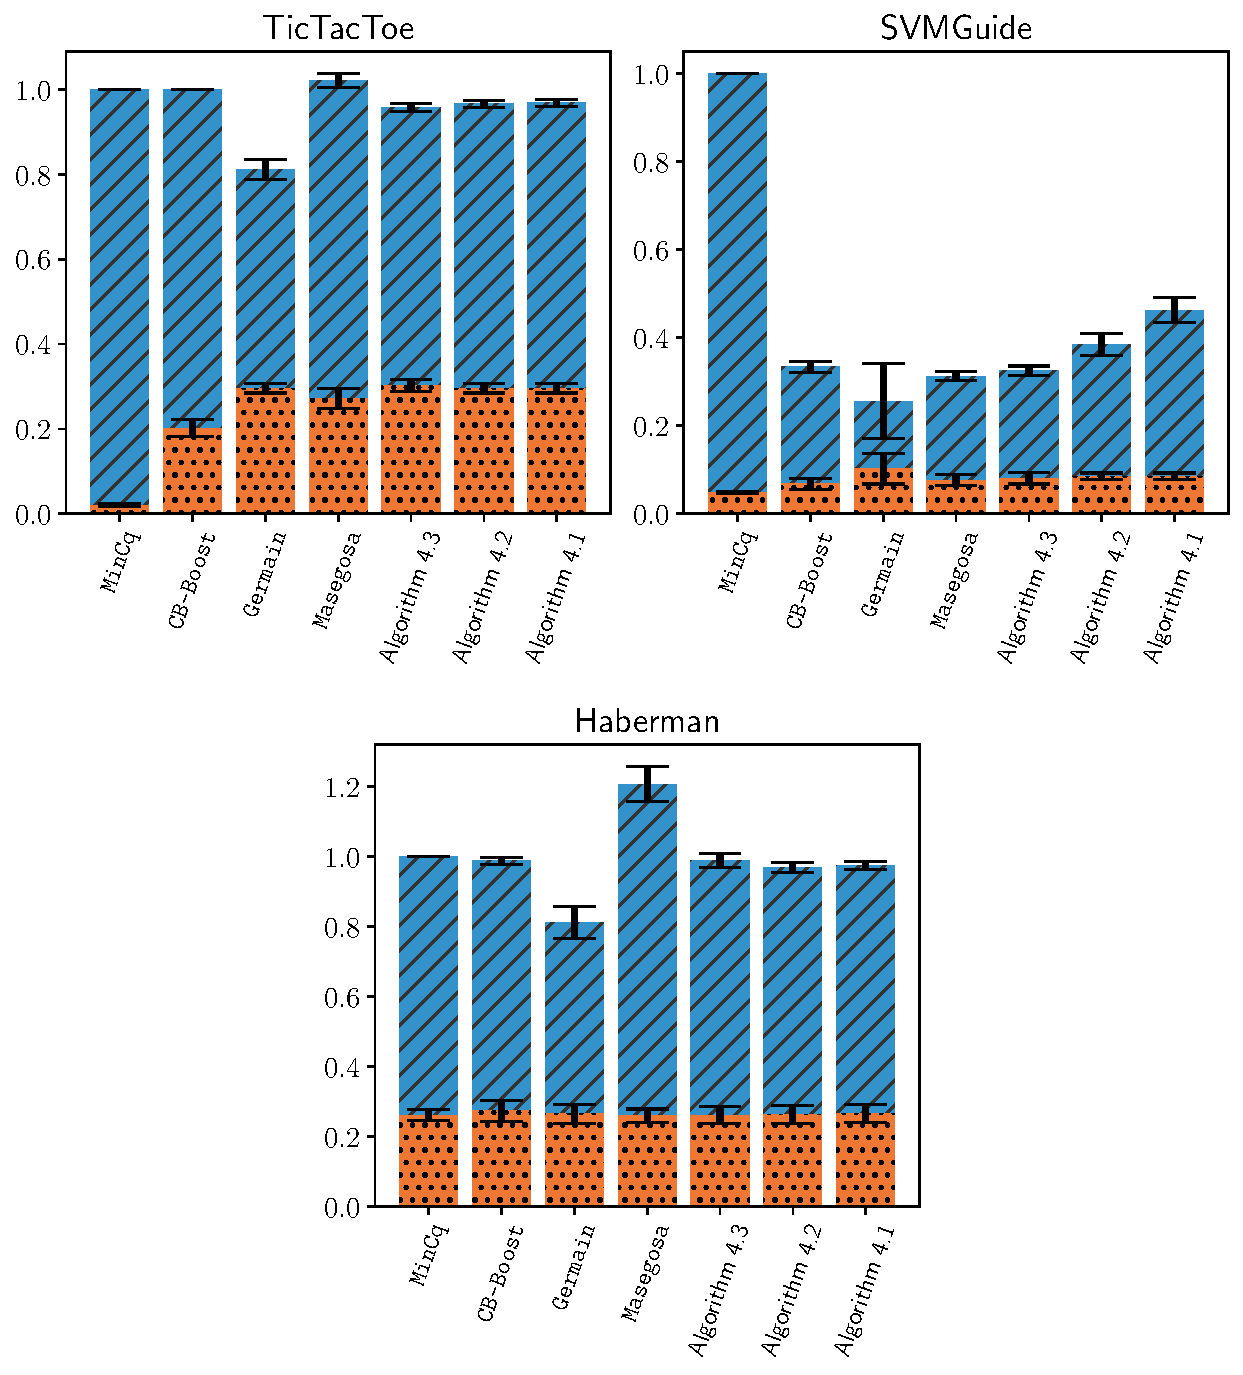
\includegraphics[width=1.0\linewidth]{chapter_4/figures/stump_binary_2.pdf}
    \caption[Comparison Between the Test Risks and the Bounds (2/6)]{
    Plot of a comparison between the test risks $\Risk_{\dT}(\MVQ)$ and the generalization bounds in the binary setting when the voters are decision stumps.
    For each algorithm, we represent the mean of the test risks in the orange bars and the bounds' mean in the blue bars.
    Additionally, the black lines are the standard deviations. 
    }
    \label{chap:mv:fig:stump-binary-2}
\end{figure}

\begin{figure}
    \centering
    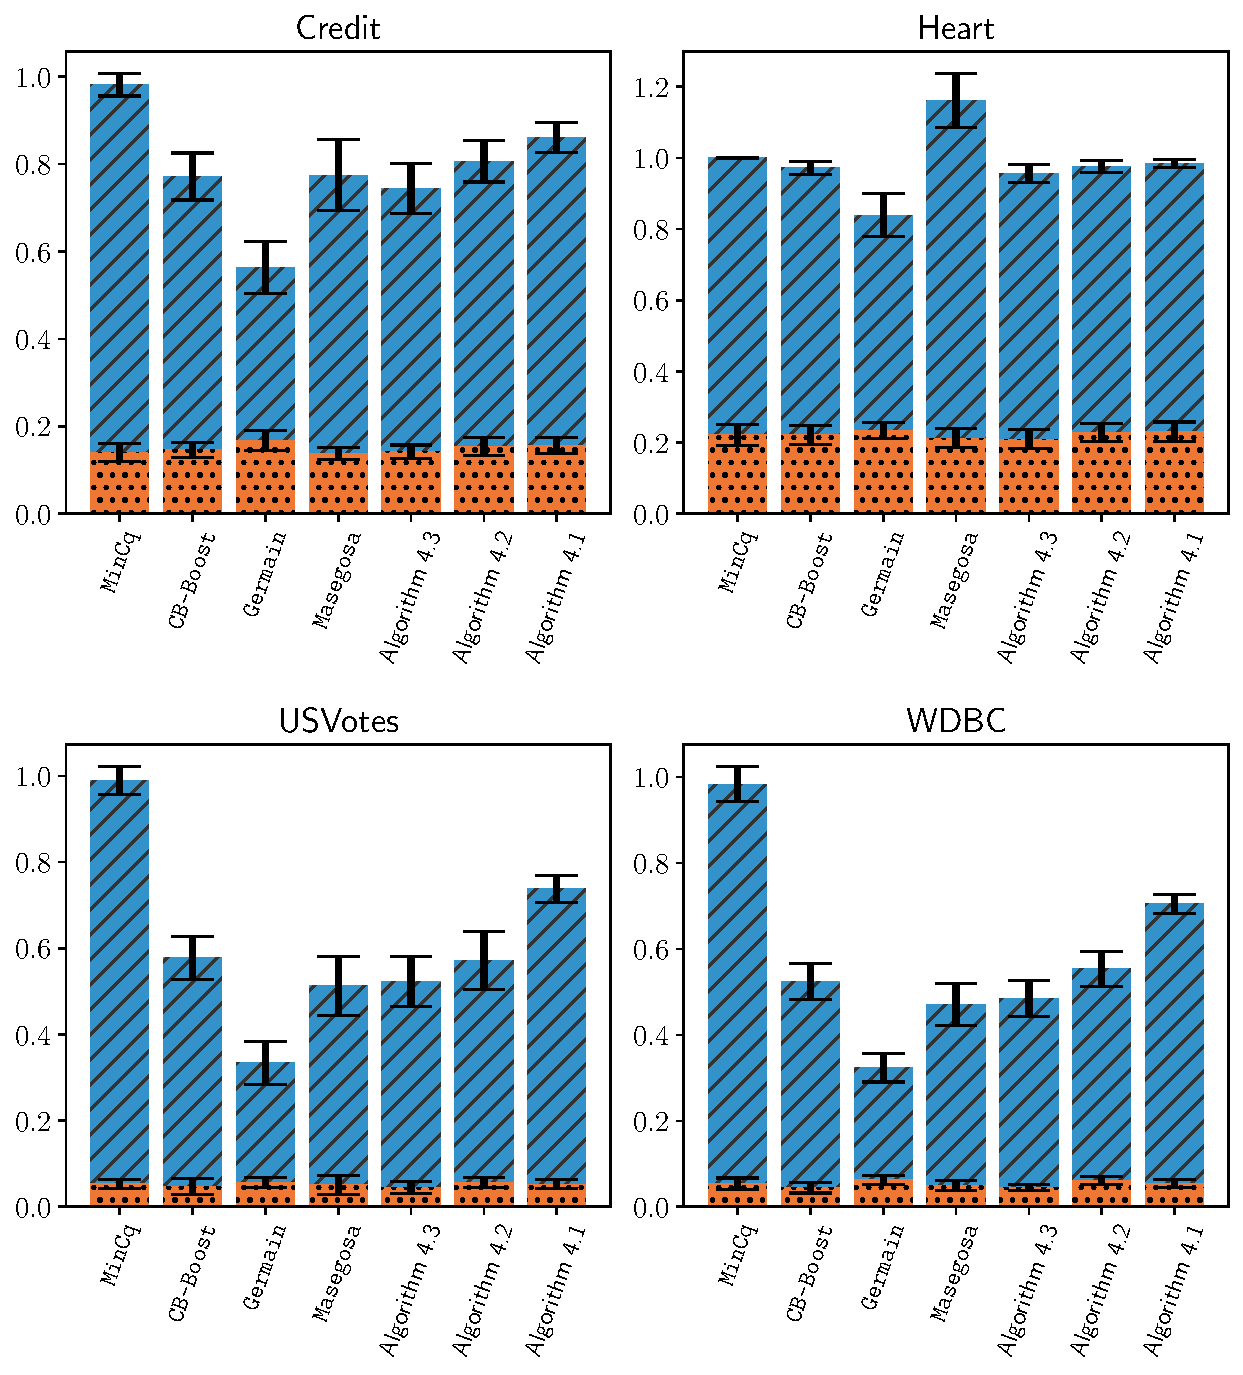
\includegraphics[width=1.0\linewidth]{chapter_4/figures/tree_binary_1.pdf}
    \caption[Comparison Between the Test Risks and the Bounds (3/6)]{
    Plot of a comparison between the test risks $\Risk_{\dT}(\MVQ)$ and the generalization bounds in the binary setting when the voters are decision trees.
    For each algorithm, we represent the mean of the test risks in the orange bars and the bounds' mean in the blue bars.
    Additionally, the black lines are the standard deviations. 
    }
    \label{chap:mv:fig:tree-binary-1}
\end{figure}

\begin{figure}
    \centering
    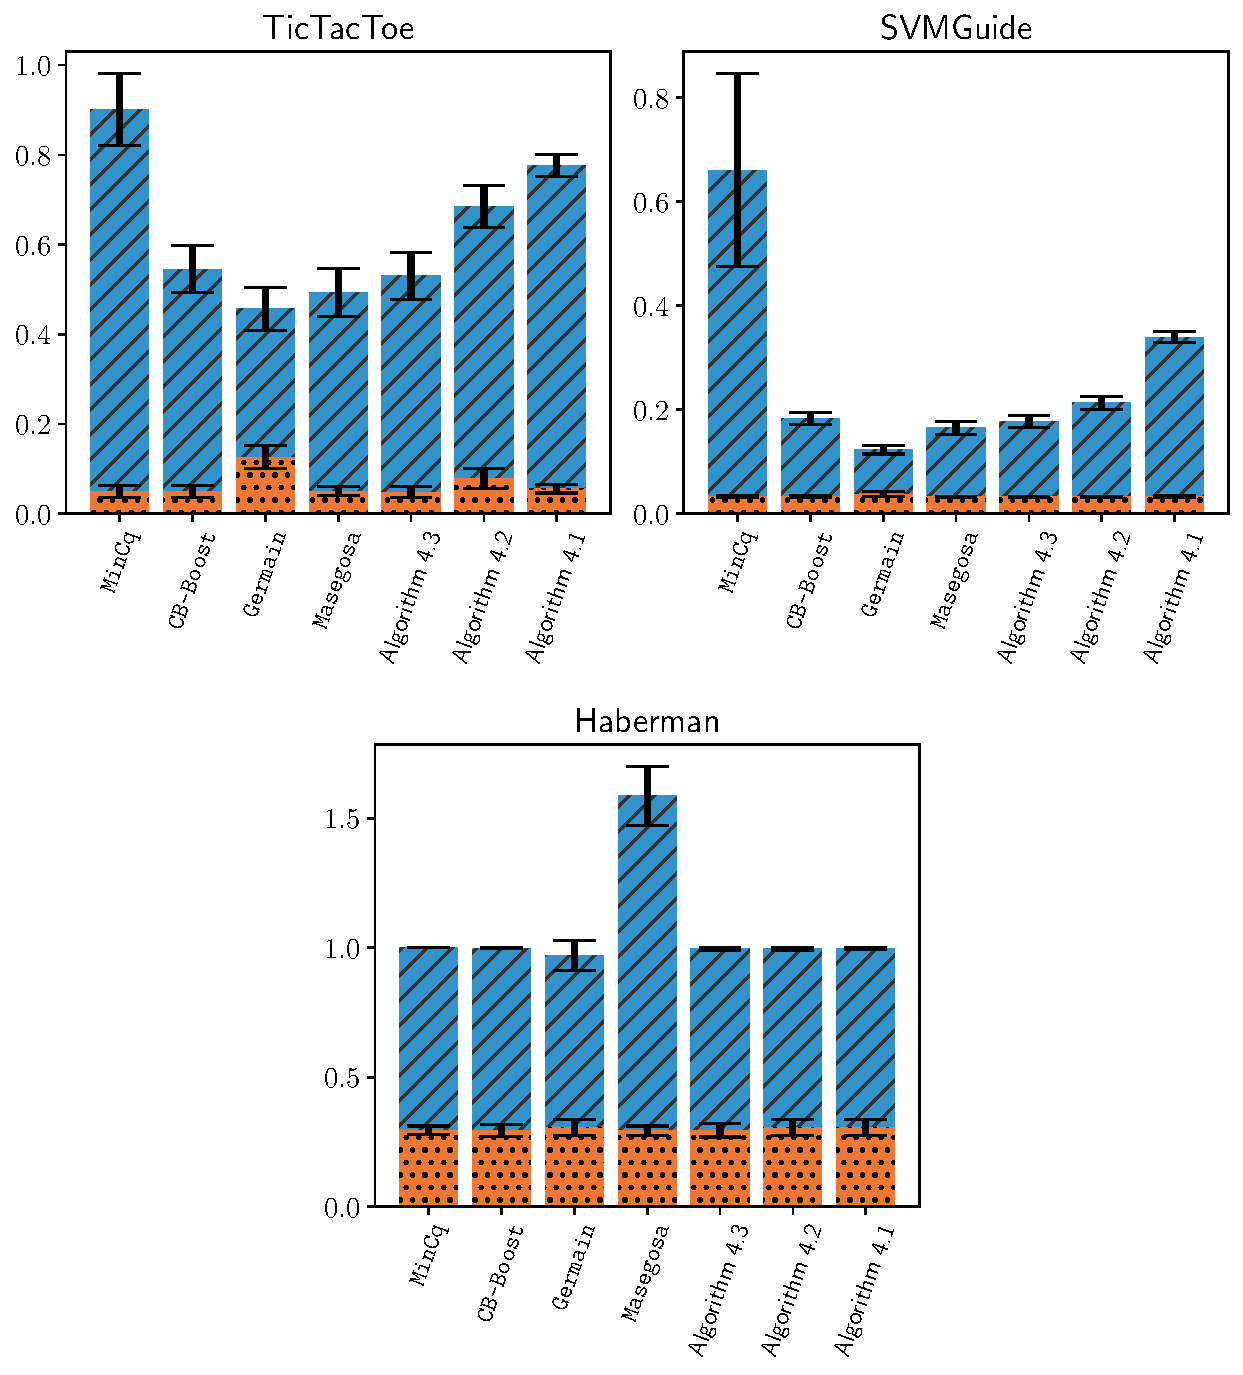
\includegraphics[width=1.0\linewidth]{chapter_4/figures/tree_binary_2.pdf}
    \caption[Comparison Between the Test Risks and the Bounds (4/6)]{
    Plot of a comparison between the test risks $\Risk_{\dT}(\MVQ)$ and the generalization bounds in the binary setting when the voters are decision trees.
    For each algorithm, we represent the mean of the test risks in the orange bars and the bounds' mean in the blue bars.
    Additionally, the black lines are the standard deviations. 
    }
    \label{chap:mv:fig:tree-binary-2}
\end{figure}

\begin{figure}
    \centering
    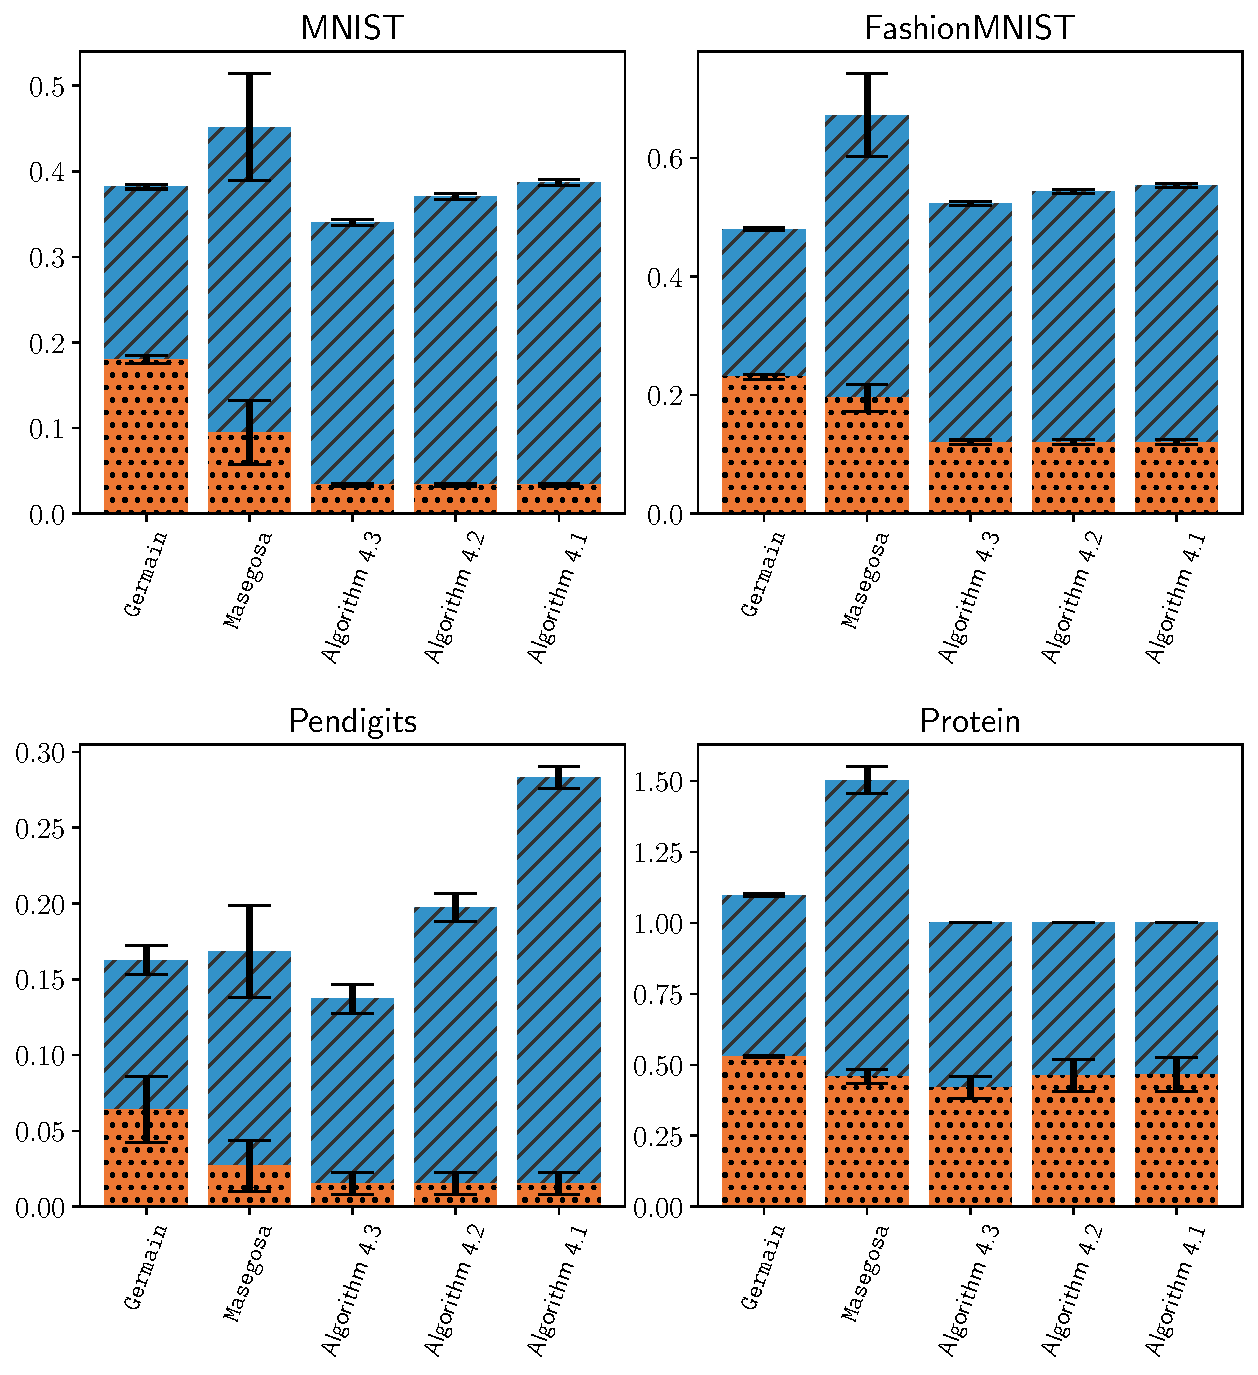
\includegraphics[width=1.0\linewidth]{chapter_4/figures/tree_multi_1.pdf}
    \caption[Comparison Between the Test Risks and the Bounds (5/6)]{
    Plot of a comparison between the test risks $\Risk_{\dT}(\MVQ)$ and the generalization bounds in the multi-class setting when the voters are decision trees.
    For each algorithm, we represent the mean of the test risks in the orange bars and the bounds' mean in the blue bars.
    Additionally, the black lines are the standard deviations. 
    }
    \label{chap:mv:fig:tree-multi-1}
\end{figure}

\begin{figure}
    \centering
    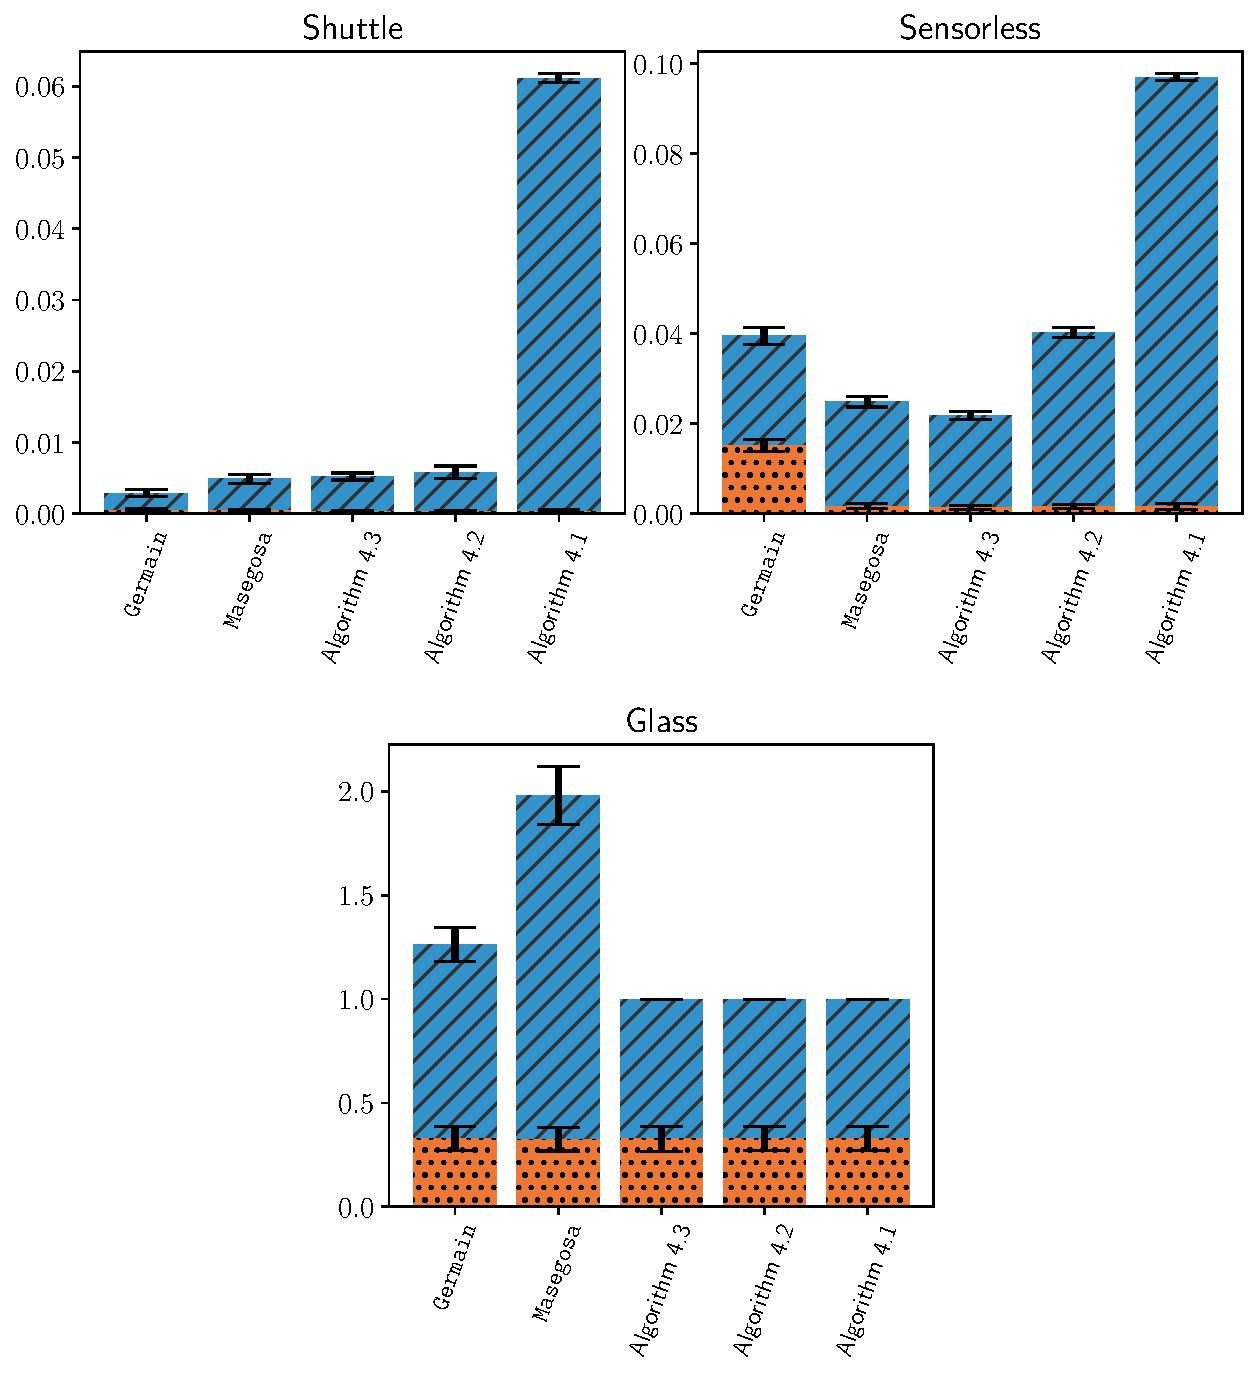
\includegraphics[width=1.0\linewidth]{chapter_4/figures/tree_multi_2.pdf}
    \caption[Comparison Between the Test Risks and the Bounds (6/6)]{
    Plot of a comparison between the test risks $\Risk_{\dT}(\MVQ)$ and the generalization bounds in the multi-class setting when the voters are decision trees.
    For each algorithm, we represent the mean of the test risks in the orange bars and the bounds' mean in the blue bars.
    Additionally, the black lines are the standard deviations. 
    }
    \label{chap:mv:fig:tree-multi-2}
\end{figure}

Our experiments have a two-fold objective: \textit{(i)} assessing the guarantees given by the associated PAC-Bayesian bounds, and \textit{(ii)} comparing the performance of the different C-bound-based algorithms in terms of risk optimization.
We introduce the setting in the following and we report in \Cref{chap:mv:fig:stump-binary-1,chap:mv:fig:stump-binary-2,chap:mv:fig:tree-binary-1,chap:mv:fig:tree-binary-2,chap:mv:fig:tree-multi-1,chap:mv:fig:tree-multi-2} the mean/standard deviation of the risks on the test set $\T$ and the bound values (with $\delta=0.05$) for 10 runs; see also \Cref{ap:mv:sec:details} for more details.
The setting of the experiments is as follows.

\paragraph{Dataset.}
We consider several binary and multi-class datasets like FashionMNIST \citep{XiaoRasulVollgraf2017}, MNIST~\citep{LeCunCortesBurges1998} and some coming from the UCI repository~\citep{DuaGraff2017}.
For each different run, we keep the same number of examples in the test or the train set as in the original split.
When there is no original split, we use 50\% of data in the training set $\S$ and 50\% in the test set (except for Sensorless where we have 15\% in the test set because the original set is large).

\paragraph{Voters.}
In the binary setting, we consider either a set $\H$ of decision trees or decision stumps that is complemented: if $\h\in\H$ then there is $\h'\in\H$ \st $\h'(\x)=-\h(\x)$ for all $\x\in\X$.
Concerning the multi-class setting, we only consider decision trees.
Indeed, having decision stumps would have resulted in too many voters.  
Following \citet{MasegosaLorenzenIgelSeldin2020}, the prior distribution $\P\in\M^{*}(\H)$ is set as the uniform distribution.
For the decision stumps, following \citet{RoyLavioletteMarchand2011,BauvinCapponiRoyLaviolette2020}, we use 10 decision stumps per feature.
For the decision trees, we follow a general setting similar to the one of~\citep{MasegosaLorenzenIgelSeldin2020}.
Moreover, $100$ trees are learned with $50\%$ of the training data (the remaining part serves to learn the posterior $\Q$).
More precisely, for each tree $\sqrt{d}$ features of the $d$-dimensional input space are selected, and the trees are learned by using the Gini criterion until the leaves are pure. 

\paragraph{Algorithms' parameters.}
To update of the posterior $\Q$ in \Cref{chap:mv:algo:mcallester,chap:mv:algo:seeger,chap:mv:algo:lacasse} is done through the COCOB-Backprop optimizer~\citep{OrabonaTommasi2017} (its parameter remains the default one).
In the binary setting, we optimize for $T=2,000$ iterations (by batch gradient descent), and in the multi-class setting, we set $20$ epochs with a batch size of $64$.
Lastly, we consider the parameter $\lambda{=}100$ for log-barrier extension $\logbar_{\lambda}()$.

\paragraph{Comparisons.}
We compare the three algorithms proposed in this chapter to the following state-of-the-art PAC-Bayesian methods for majority vote learning.
\begin{itemize}
    \item We compare with the algorithm proposed by \citet{MasegosaLorenzenIgelSeldin2020} that optimizes a PAC-Bayesian bound on $\Risk_{\D}(\MVQ) \le 4e_{\D}(\Q)$ (\Cref{chap:pac-bayes:theorem:4joint}); see Theorem~9 and Appendix~G of \citep{MasegosaLorenzenIgelSeldin2020} for a description of this algorithm that we denote by \algomasegosa.
    For \citeauthor{MasegosaLorenzenIgelSeldin2020}'s algorithm, we kept the original parameters.

    \item Our algorithm to optimize the PAC-Bayesian bound on $\Risk_{\D}(\MVQ) \le 2r_\D(\Q)$ (\Cref{chap:pac-bayes:theorem:2gibbs}) recalled in \Cref{chap:mv:theorem:pb-2gibbs} and derived by \citep[PAC-Bound 0]{GermainLacasseLavioletteMarchandRoy2015}.
    Even though \citep{GermainLacasseLavioletteMarchandRoy2015} does not optimize the bound, we denote this algorithm by \algogermain.
    The algorithm is similar to \Cref{chap:mv:algo:seeger}, but without the numerator of the C-Bound (\ie, the disagreement); more details are given in \Cref{ap:mv:sec:pb-2gibbs}.

    \item In the binary setting only, we compare with \mincq \citep{RoyLavioletteMarchand2011} and \cbboost \citep{BauvinCapponiRoyLaviolette2020} that are based on the minimization of the empirical C-Bound $\CBound_{\dS}(\Q)$.
    Indeed, these algorithms are developed for this setting only.
    For comparison purposes and since \mincq and \cbboost do not explicitly minimize a PAC-Bayesian bound, we report the bound values of \Cref{chap:mv:theorem:new-cbound-lacasse} instantiated with the models learned;
    Moreover, for \mincq, we select the margin parameter among $20$ values uniformly spaced between $[0,\tfrac{1}{2}]$ by 3-fold cross validation. 
    For \cbboost, which is based on a Boosting approach, we fix the maximal number of boosting iterations to $200$.
\end{itemize}

\subsection{Analysis of the Results}

When comparing only the PAC-Bayesian C-Bounds, we observe in \Cref{chap:mv:fig:stump-binary-1,chap:mv:fig:stump-binary-2,chap:mv:fig:tree-binary-1,chap:mv:fig:tree-binary-2,chap:mv:fig:tree-multi-1,chap:mv:fig:tree-multi-2} that \Cref{chap:mv:algo:mcallester} provides the worst bound.
\Cref{chap:mv:algo:lacasse} provides usually tighter bounds than \Cref{chap:mv:algo:mcallester,chap:mv:algo:seeger} except for Harberman and USVotes.
We believe that \Cref{chap:mv:algo:lacasse} provides lower bounds than \Cref{chap:mv:algo:seeger} because the \citeauthor{LacasseLavioletteMarchandGermainUsunier2006}'s approach bounds simultaneously the joint error and the disagreement.
\Cref{chap:mv:algo:lacasse} appears then to be the best algorithm among our three self-bounding algorithms that minimize a PAC-Bayesian C-Bound.
Moreover, \Cref{chap:mv:algo:lacasse} gives usually the lowest true risks or it is comparable to the two other algorithms.\\

Compared to the baselines, \algogermain~gives usually the lowest bounds among all the algorithms, but at the price of a large test risk.
This clearly illustrates the limitation of considering \textit{only} the Gibbs risk as an estimator of the majority vote risk: as discussed in \Cref{chap:pac-bayes:sec:surrogate}, the Gibbs risk is an unfair estimator since an increase in the diversity between the voters can have a negative impact on the Gibbs risk.\\
Second, compared to \citeauthor{MasegosaLorenzenIgelSeldin2020}'s approach, the results are comparable.
This behavior was expected since minimizing the bound of~\citet{MasegosaLorenzenIgelSeldin2020} or the PAC-Bayesian C-Bound boils down to minimize a trade-off between the risk and the disagreement.
Third, in the binary setting, compared to empirical C-bound minimization algorithms, we see that \Cref{chap:mv:algo:lacasse} outputs better results than \cbboost and \mincq for which the difference is significative, and the bounds are close to $1$ (\ie, non-informative).
Optimizing the risk bounds tends to provide better guarantees that justify that optimizing the empirical C-bound is often too optimistic (as done in \cbboost or \mincq); we provide in \Cref{ap:mv:sec:joint-disa} an illustration of the different solutions obtained from the algorithms.\\

Overall, from these experiments, our \Cref{chap:mv:algo:lacasse} is the one that provides the best trade-off between having good performances in terms of risk optimization and ensuring good theoretical guarantees with informative bounds.
Moreover, in \Cref{ap:mv:sec:time} we show that \Cref{chap:mv:algo:lacasse} has a higher computation time than the others algorithms.
This makes \Cref{chap:mv:algo:seeger} a good trade-off between ensuring good theoretical guarantees and having a low computation time.

\section{Conclusion and Summary}

This chapter presents learning algorithms that minimize the majority vote's risk with PAC-Bayesian generalization bounds based on the C-Bound. 
More precisely, we propose solving three optimization problems, each derived from an existing PAC-Bayesian bound.
Our methods belong to the class of {\it self-bounding} learning algorithms~\citep{Freund1998}: the learned predictor comes with a tight and statistically valid risk upper bound.
Our experimental evaluation has confirmed the quality of the learned predictor and the tightness of the bounds with respect to state-of-the-art methods minimizing the C-Bound.\\

As we said before, no algorithm minimizes the {\it empirical} C-Bound in the multi-class setting.
One of the reasons is that it is not easy to find a convex program like for \mincq or \pmincq algorithm.
Hopefully, thanks to the deep learning framework, minimizing the C-Bound is possible even without convexity through a stochastic gradient descent algorithm (as we show in \Cref{chap:mv-sto} in the binary setting).
Hence, in the future, we plan to explore more the minimization of the C-Bound.\\

However, one drawback of the PAC-Bayesian C-Bounds and the other ones of the literature is that the majority vote true risk is not directly minimized: we need surrogates such as the Gibbs risk, the disagreement, or the joint error.
Indeed, the C-Bound is already an upper bound on the true risk, which makes the PAC-Bayesian C-Bound even looser, thus, these generalization bounds cannot be tight.
To avoid this issue, we bound the {\it expected} true risk of the majority vote.
This is done in the next chapter: we {\it (i)} introduce the {\it stochastic} majority vote that samples a distribution $\Q$ for each prediction, and we {\it (ii)} provide guarantee on the true risk for this classifier.
As we will see, our obtained (PAC-Bayesian) guarantee is differentiable, and we can derive self-bounding learning to learn such a classifier.